\chapter{Software Development in ROS2}\label{c:ros}

Robotic systems have emerged into several scenarios, where its usage ranges between basic processes automation, up to full performance over critical tasks, consequently causing the complexity increase in these domains. Concerning the complexity behind writting software code, due to the widely variety presented in the robot's hardware as in fields of action \cite{cousins2011exponential}, Robotic Operation System (ROS) presents itself as a middleware system, created to facilitate robotic systems development.

In ROS, software flexibility was valued above all else, meaning that values like security were not duly valued, so ROS-based applications tend to face increased security risks, exposing the whole robotic network. As ROS became a standard for many robotic systems, and due to the scale and scope of the robotics growth, security ensurance must be addressed as a developing priority. \cite{diluoffo2018robot, kim2018security}

The upgraded version of ROS, Robot Operating System 2 (ROS2), presents itself as a framework for developing robotic systems, supported by a standard, the Data Distribution Service (DDS), where multiple middleware implementations are built over this standard, providing ROS applications multiple DDS-based specfications, as well as valued Quality of Service (QoS) settings over the transport configuration. 

The DDS-Security specification \cite{dds-s}, embedded by every DDS implementation supported by ROS, supplies multiple plugins regarding the security domain. As result, ROS2 yields a wider command toolset compared to the former version of ROS, as they bring forth to a toolset, the Secure Robot Operating System 2 (SROS2) toolset, concerning the security functionality that DDS-Security plugins offer.

This chapter introduces necessary background information over the major concepts on which this thesis rests. First, it is presented a detailed introduction to the concepts around Robot Operating System (ROS), as well as the evolution approach that ROS faced towards providing security to its deployed systems. Regarding this goal, Data Distribution Service (DDS) and its integration on Robot Operating System 2 (ROS2) must be contextualized beforehand.


\section{Architecture Considerations}

The Robot Operating System was created by a collaborative open-source community, that has undergone rapid development \cite{cousins2011exponential}, to contribute in the advancement of cyber physical systems, serving as developer enhancer for the world of robotic applications. \cite{diluoffo2018robot, intro-ros}

% Although Robot Operating System furnishes services, such as hardware abstraction, low-level device control and control over message-passing between processes, ROS can not be perceived as a proper operating system, in the sense of process management and scheduling. However, it has a significant impact on the deployed application's performance, with highly complex effects on timing, inevitably affecting the application's runtime behaviour. In result, the impact of the underlying operating system scheduling is over exceeded by ROS. \cite{intro-ros, casini2019response} 

Fundamentally, ROS is a middleware, as it provides a custom serialization format, a custom transport protocol as well as a custom central discovery mechanism, presenting itself as a distributed layer between the top application layer and the operating system layer. ROS was designed to provide as much as modularity and composability to the application layer \cite{casini2019response} as possible, allowing ROS applications to be built over several software modules, as independent computing processes called \textit{nodes}, that compose together to fulfill the deployment characteristics of the corresponding robot. \cite{maruyama2016exploring} 

\subsection{Former Architecture}


% The communication approach that ROS implements to perform data exchange between nodes is based on a publish-subscribe model, based on TCPROS \cite{tcpros} and UDPROS \cite{udpros}, that makes use of TCP and UDP sockets, respectively. \cite{maruyama2016exploring} The data transportation is done by introducing the \textit{message} definition, which commonly characterizes every data structure concerning the information exchange between ROS participants. 

The former communication architecture supported by ROS focused on a centralization perspective, as it had a implementation of a \textit{Master node}, that controlled every aspect of the communication establishment. Every information exchange between nodes had to go through this master, as these nodes must also be able to address the ROS Master's location.

Due to the sheer wide capabilities controlled by the master, this centralization approach fits the purposes of a research tool, as it is simpler to monitor and analyse the system behaviour. This communication architecture, however, does not scale well since it is heavily reliant on the master node's availability, making it unsuitable for safety-critical and real-time applications. If the master fails, the entire system fails, representing a single point of failure and a huge performance bottleneck.

\begin{figure}[H]
  \centering
  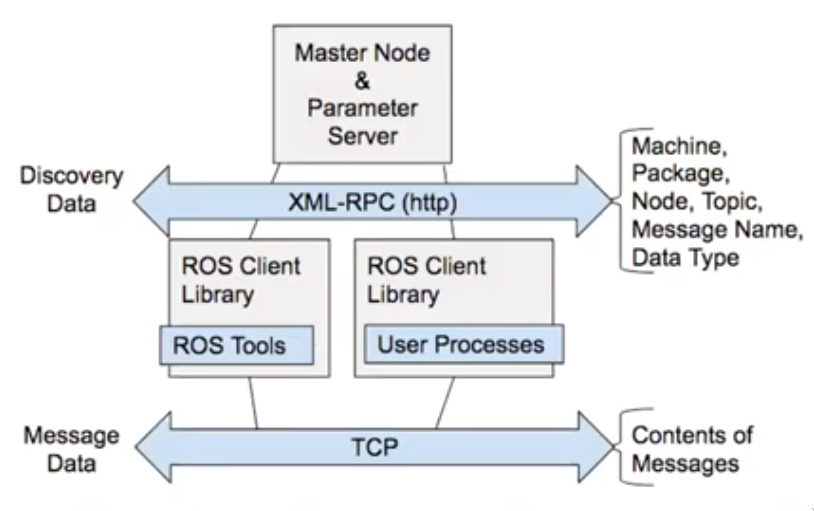
\includegraphics[width=0.6\linewidth]{images/former-ros1-architecture.png}
  \caption{Robot Operating System architecture.}
  \label{fig:ros1-architecture}
\end{figure}

Many research communities tried to fix these real-time issues by proposing potential solutions, while supporting the same architecture design. However, these solutions did not fully accomplished the needs of real-time applications. So, it became clear to the ROS community that the framework had architectural limitations that could not be rearranged using the same design approach. \cite{maruyama2016exploring}

Robot Operating System 2 comes as a complete refactoring of ROS, with the aim of increase the framework's real-time capabilities, by allowing the development of time-critical control over ROS, as it moves away from the former architectural design towards the implementation of an external middleware that can support the production needs of the outgrowing robotic systems. \cite{kim2018security, casini2019response}

%This lead to the creation of \textbf{ROS2}, which continues to provide a simple, uniform message passing interface to allow components to communicate with each other, now implemented using the Data Distribution Service (DDS) communication protocol as middleware. This means that there is no need to implement a master, making the system fully distributed. The discovery process between nodes is distributed and guaranteed by DDS, giving theses nodes the capacity to discover other nodes. Considering that there is no ROS Master implemented, the approach when dealing with the parameters also changed. Instead of having a global parameter server, in ROS2 each node declares and manages its own parameters. All these aspects related to ROS2 will be later discussed.

% The Robot Operating System 2 (ROS2) was developed towards tackling the former ROS architecture's issues. Although ROS2 continues to provide a simple, uniform message passing interface to allow components to communicate with each other, instead of implementing their own middleware specification, Data Distribution Service (DDS) communication protocol is implemented as an abstract middleware interface, through which serialization, transport and discovery are guaranteed. % This implies that adding and integrating a new component into an existing system remains reasonably simple for a ROS developer.

\subsection{Data Distribution Service}

The Data Distributed System \cite{3}, simply known as DDS, is a Object Management Group (OMG) middleware standard, resulted from the need of better interoperability between different vendors middleware frameworks, directly addressing data communication between nodes that belong to a \textit{publish-subscribe} communication architecture, for real-time and embedded systems. %, that relies on a data-centric approach. 
            
% A middleware, such as DDS, is a software layer that lies between the operating system and the Application layer. \cite{dds-what-is} 
A middleware, such as DDS, aims to ease the complexity behind creating each sytem's own middleware, by handling relevant aspects like network configuration, communication establishment, data sharing and low-level details. As a result, system developers can mainly focus on their applications purposes, rather than concerning about information moving across levels. \cite{dds-what-is} 

% DDS disposes a software API supported by a rich documentation about its exact behaviour. By furnishing this specification, it enables third parties applications, such as ROS, to implement this middleware, while auditing and understanding matters are covered by its documentation. 

% Data centricity
% The architecture approach is based on a concept named \textit{Data-Centric}, where the message-data itself is the focal point. Here, the infrastructure formally defines the data and imposes rules over it, with the continuous awareness of the contents in the data space, as data is properly delivered to the applications which quest for it, saving bandwith and processing power. \cite{3} Rather than forcing each application to deal with this complexity of defining the data space, DDS directly implements and provides controlled, managed, secure data sharing. \cite{pardo2005introduction}

DDS uses the Data-Centric Publish Subscribe (DCPS) model as its communication model approach. DCPS is based on a \textit{publish-subscribe pattern}, where the \textit{data-centric} messaging technique is implemented. It conceptually creates a virtual \textit{global data space}, acessible by any DDS-based application, where data is properly delivered to the applications which quest for it, saving bandwith and processing power. \cite{3, pardo2005introduction} A domain participant enables an application to participate in the global data space, either as a \textit{publisher} or as a \textit{subscriber}, according to their role on data exchange. \cite{maruyama2016exploring, alaerjan2017modeling, dcps-rtps} 

% In a data-centric architecture, the infrastructure formally defines the data and imposes rules over it, with the continuous awareness of the contents in the data space, as data is properly delivered to the applications which quest for it, saving bandwith and processing power. \cite{3, pardo2005introduction} % Rather than forcing each application to deal with this complexity of defining the data space, DDS directly implements and provides controlled, managed, secure data sharing. \cite{pardo2005introduction}

% A domain participant enables an application to participate in the global data space, either as a \textit{publisher} or as a \textit{subscriber}, according to their role on data exchange. A publisher is composed by \textit{Data Writers}, where each of them publishes data to a corresponding \textit{topic}. A \textit{topic} represents the data space objects through which data is handled. A \textit{Data Reader}, complementing the role of the data writer in the DCPS data transportation, declares the intent to subscribe to the topic. A subscriber can be composed by one or more data readers. \cite{alaerjan2017modeling, dcps-rtps}

\begin{figure}[H]
    \centering
    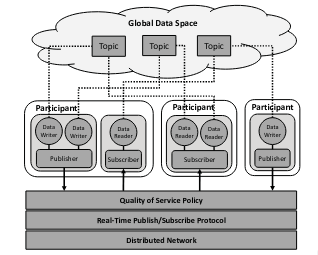
\includegraphics[width=0.6\linewidth]{images/dcps-model.png}
    \caption{DDS architecture: DCPS model with RTPS. Extracted from \cite{maruyama2016exploring}.}
    \label{fig:dcps-model}
\end{figure}

To properly adress the data transportation through physical network, DDS offers a wire specfication protocol called Real-Time Publish-Subscribe Wire Protocol (RTPS) \cite{rtps}, providing automatic discovery between participants. This protocol also works under a \textit{publish-subscribe} policy over best-effort transports, where data transmission between endpoints is handled. \cite{yun2017data} RTPS allows multiple applications, that could differ on their used DDS implementations, to interoperate with each other as network domain participants. \cite{dcps-rtps, alaerjan2017modeling} % Towards easing the communication establishment, RTPS provides a set of discovery services, allowing the automatic discovery between participants. \cite{dcps-rtps}

Furthermore, RTPS was designed to make use of \textit{Quality of Service} profiles, where multiple transport policies can be specified that, by default, DDS does not support. This approach offers flexibility over communication configuration and development versatility, allowing the developer to specify whatever QoS satisfies its system's communication needs. \cite{alaerjan2017modeling, diluoffo2018robot, maruyama2016exploring} % For instance, as multiple DDS vendors are built over the UDP \cite{udp} transport protocol, which does not feature reliable delivery of data, transport reliability, often required by real-time environments, can be ensured by specifying the realiability's corresponding QoS policy into the RTPS communication layer. Besides, QoS profiles also enables security deployment into the transport configuration. 


% Additionally, each domain entity manages the data according to the Quality of Service profiles speficified over the RTPS protocol, that is used over the transportation process as a policy. Applications within the network are then generated as DDS domain participants, with regard of the transport QoS policies. \cite{alaerjan2017modeling, maruyama2016exploring} 

Briefly speaking, DDS leverages the premise of a transport-independent virtualized Data Bus to address network resources' distribution, in which stateful data is distributed through the network. The involved applications can acess this data in motion, representing an architecture with no single point of failure, respectively enabling a realiable way of ensuring data integratity. Consequently, by adopting this approach, the load on the network is independent of the number of applications, making it easily scalable. % DDS communications are also governed with explicit \textit{Quality of Service} settings, that allows the system to manage and monitor which applications are able to communicate in which ways with the Data Bus and with each other. 

\begin{figure}[H]
    \centering
    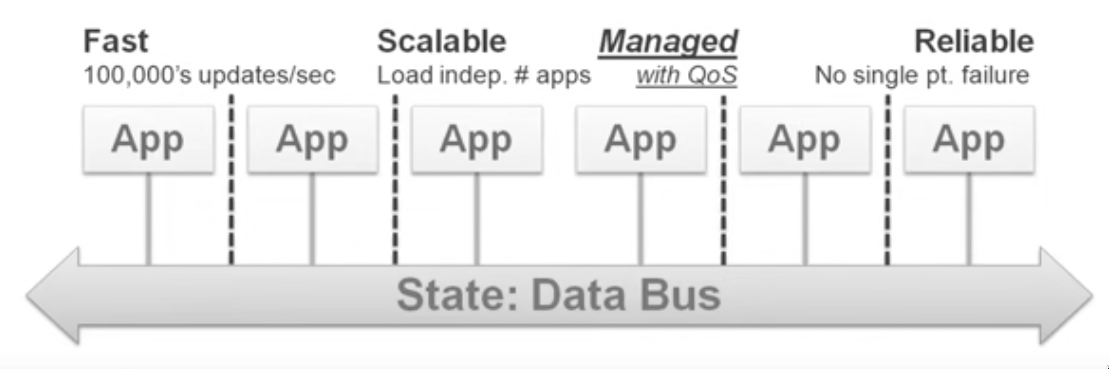
\includegraphics[width=0.6\linewidth]{images/dds-architecture.png}
    \caption{Data Distributed System architecture in a nutshell.}
    \label{fig:dds-architecture-nutshell}
\end{figure}

% Introduzir as implementações e DDS specifications

\subsection{ROS2-DDS Architecture}

As previously stated, the Robot Operating System 2 was developed to address the lack of support for real-time systems that the former ROS provided, mainly due to its architecture design that relied on their own middleware specification. To address this, ROS2 middleware approach is built upon the DDS framework \cite{maruyama2016exploring}, leveraging DDS for its messaging architecture, where communication and transport configuration are handled. % As a result of the DDS integration, ROS2 applications are actually considered DDS applications, meaning that is possible to interoperate both native DDS applications and ROS applications, providing flexible compatibility.

%By relying on an outside middleware, the modularity approach that ROS makes use of, where multiple modules should be applied when needed, while reducing the number of dependencies attached, highly depends on the middleware implementation that is being used. 
As far as dependencies are concerned, DDS implementations have light sized dependencies, often related to language implementation libraries, easing the complexity behind installing and running dependencies for ROS developers. \cite{ros-on-dds}

The middleware's on-top layer regards the ROS client library (\textit{rcl}), already implemented in the former ROS architecture. This layer accounts the availability of ROS concepts to the Application layer, as it provides APIs to ease the software implementation by ROS developers. \cite{ros2documentation} As ROS aims to support different programming languages over the same computing context, each language-specficic API must have its corresponding client library (\textit{rclcpp} regarding \textit{C++} and \textit{rclpy} regarding \textit{Python}). The \textit{rcl} accounts these client libraries by abstracting their specification, reducing code duplication.   
\cite{rcl, casini2019response}

% ROS2 middleware implements an interface layer on top of DDS, called \textit{ROS client library} (RCL), alread which hides much of the complexity of DDS specification API, offering a more friendly approach for the ROS users. However, it still provides access to the underlying DDS implementation for users that might want to integrate different DDS implementations for their use cases.

\begin{figure}[H]
    \centering
    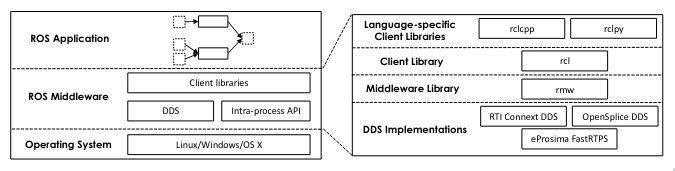
\includegraphics[width=\linewidth]{images/ros2-architecture.png}
    \caption{ROS2 framework architecture.}
    \label{fig:ros2-architecture}
\end{figure}

Towards supplying a wide range of configurations back to application layer, to vastly cover the robotic applications needs, ROS2 aims to support multiple DDS implementations, in which these implementation's API specification might differ from each other (currently, FastRTPS by eProsima, Connext by RTI, and Vortex OpenSplice by Adlink). It should be noted that the DDS implementations are low-level of abstraction, strictly defined by its corresponding vendor's API. DDS only defines fundamental procedures at a higher degree of abstraction.  

In order to abstract \textit{rcl} from the specifications complexity of these implementations APIs, an DDS-agnostic interface is being introduced, the \textit{rmw} (ROS MiddleWare) interface \cite{casini2019response}, allowing portability among DDS vendores, which consequently enables ROS developers to interpolate DDS implementations, based on their applications needs during runtime. The information flow through the middleware layer is done over structure mapping between ROS and DDS data models, addressed by the \textit{rmw}, regarding the DDS implementation that is being considered at runtime.

% This layer could be removed, if there was no need to use more than one DDS implementation. But this is not the wanted scenario, since it is way more practical to switch the DDS implementation depending on the application needs. 
% The former version of ROS, depicted on left hand-side of the picture \ref{fig:ros2-architecture}, already provided this abstract layer, that was customized and implemented by ROS client library, which allowed the communication between the Application Layer, in hwich the Master node was implemented, and the communication protocols. However, the capabilities offered by this middleware are significantly lower than ROS2 middleware, due to the DDS integration, as well as the fail to support the needs of multiple systems.

% As stated, ROS client library hides the complexity of the DDS specification API from the developer. 
% Since the \textit{rcl} layer works under ROS structures, in order to keep the passing of information through the middleware layer, a structure mapping between ROS and DDS must occur in the rmw interface, regarding the DDS implementation that is being considered at runtime. \cite{casini2019response} The data structure mapping between ROS and DDS must account the preservation of the former ROS messages' structure. The \textit{rcl} layer works under the ROS messages' \texttt{.msg} files so, these messages must be converted into messages' \texttt{.idl} files, to be handled by the DDS's RTPS wire protocol. \cite{ros-on-dds} Then, the reverse process must be ensured as well, to fully complete the information flow, where data must be converted back to ROS structures before being returned to the \textit{rcl}.

\subsection{Computation Graph}

From a logical perspective \cite{casini2019response}, ROS applications are composed of many software modules that operate as computation nodes, allowing its participation into the ROS global data space. The primarily use of publish-subscribe model approach as communication type, through \textit{message-passing} patterns, confers additional concept complexity to the application architecture, where the latter can be naturally represented as a \textit{computation graph}. 

The application's computation graph presents itself as a graphical network, where runtime named entities have their unique role when it comes to data distribution. The mainly used network entities are \textit{Node Instances}, \textit{Topics} and \textit{Interfaces}, which will be covered in this presented section.

\subsubsection{Node Instances}

The application development is done over package orchestrating, where each logically represents a useful software module. Packages might be compromised by numerous \textit{nodes}, that can be perceived as processes that will likely perform computation over the network. It is worth mentioning that, nodes can be connected within a single package or between multiple packages, as they are built over their corresponding packages.

The network is comprised of many nodes, running simultaneously and exchanging data between them, where each node addresses its corresponding network module purpose. Fault tolerance features are guaranteed as nodes have their corresponding unique name, allowing communication in an unambiguous manner, which confers a suitable approach when developing a complex robotic system.

For instance, consider a well-known example called \texttt{TurtleSim}, which is a simulator typically used for learning ROS, mainly composed by \textit{two nodes}, that perform together towards moving a turtle. Additional nodes were implemented, in order to add complexity to the current network, as to later support security as a proper example. % The ROS2 command toolset allows node launching using the \textit{run} keyword, in which both the node's namespace and its corresponding package must be passed as arguments.

\begin{lstlisting}[title={The \texttt{TurtleSim} node list.}]
/multiplexer
/random
/turtle_teleop_key
/turtlesim_node
\end{lstlisting}

\subsubsection{Communication}

Message-passing models is the primary means by which nodes communicate with one another. The \textit{message} definition is a well-typed data structure, which commonly characterizes every data structure concerning the information exchange between nodes. A message is defined by its data type, also known as its \textit{interface}, which can either be primitive (integer, string, boolean), or defined by a complex data structure, where multiple data types are assigned to their corresponding variables. 

\begin{lstlisting}[title={\texttt{Twist.msg} interface file that is used to trigger the turtle movement.}]
    Vector3   linear
    Vector3   angular
\end{lstlisting}

ROS computation graph provides \textit{three} different ways of establish node communication, those being \textit{Topics}, \textit{Actions} and \textit{Services}, where each one has its different corresponding interface, specified in different folders with unique namespaces. 

% Considering the \texttt{TurtleSim} example, the main message that is used to trigger the turtle movement, is composed by multiple data movement variables regarding the linear and circular movement of the turtle. The interface is called \textit{Twist} and it is a ROS predefined geometry message.

% \begin{lstlisting}[title={\texttt{Twist.msg} interface file that is used to trigger the turtle movement.}]
% Vector3   linear
% Vector3   angular
% \end{lstlisting}

\textit{Topics} are perhaps the most common method, naturally perceived as middle-communication buses, over which messages is passed through. As semantic approach, communication through topics is handled by the publishing-subscribing pattern. A node publishes the message to any number of topics, that are then subscribed by nodes that want to get access to that message. Topics provide a multicast routing scheme, where publish data is casted into the multiple nodes that are subscribed to the topic. 

A specific \textit{topic} is created upon specifying its entity name over either a publisher or a subscriber callback instance. Whenever a node creates a publisher, intentionally instantiated to publish a message through a specified topic, \textit{roscore} is used to advertise the latter, enabling message passing to the corresponding topic subscribers. Message processing is done via the node's callback functions, which are activated upon message receipt, as it can also be utilized for publishing purposes. \cite{casini2019response} % After building and executing the node, their associated topics are created. % The available topics can be listed by running the predefined ROS command \texttt{ros2 topic list}.

\begin{figure}[H]
        \centering
        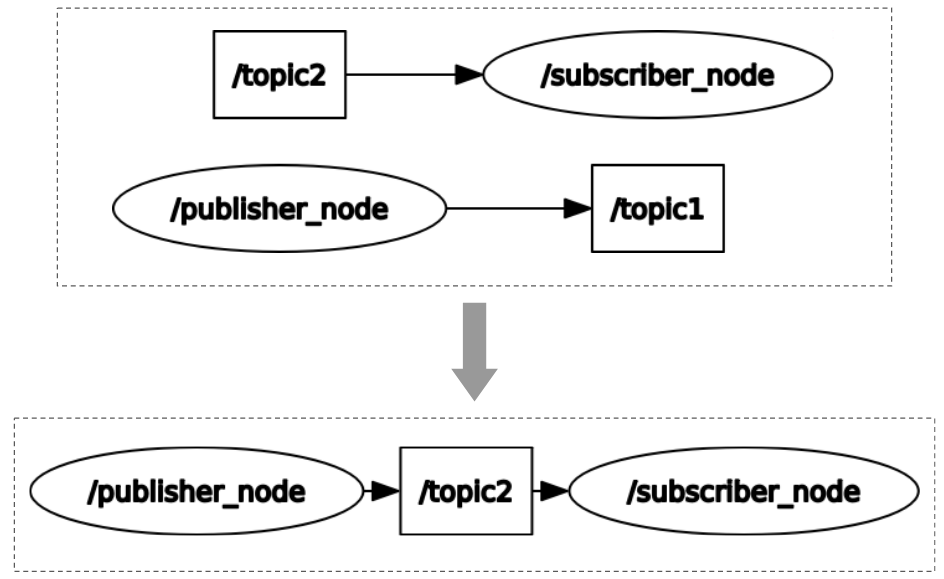
\includegraphics[width=0.4\linewidth]{images/ros2-topics.png}
        \caption{ROS2 communication behaviour over \textit{topics}.}
        \label{fig:ros2-topics}
\end{figure}

% Addressing data exchange over nodes implemented with no associated namespace, the configuration is straightforward, in which their respective subscriber and publisher instances must have the same topic's name instantiated. Whereas, if the nodes are specified over different namespaces, their topic's name will differ, so a technique of \textit{remapping} must be used.

% \begin{lstlisting}[title={The \texttt{TurtleSim} topic list.}]
% /high_topic
% /low_topic
% /main_topic
% \end{lstlisting}

% The topic list related to the \texttt{TurtleSim} example is depicted above. The 3 listed topics are vital for the communication process, and they are all managed by the \texttt{multiplexer} node. % This happens because remapping between topic names is used to establish communication between packages, as explained above. 


\subsubsection{Launch Files}

A conventional way of deploying a ROS appliaction is through the use of \textit{launch files}, enabling the multi-configuration over entire robotic applications, where network involved nodes can be individually pre-configurated. Therefore, ROS makes use of the \textit{roslaunch} to automatically initialize the whole newtork, simultaneously launching each node. This provides a simpler way of monitoring the system nodes.

Additional node configuration, such as name remapping and parameter adjustments, can be specified under the \textit{args} tag, which offers great functionality to the launching process. 

Distinctive namespaces allow the system to start the nodes, without any name nor topic name conflicts. However this technique has some flaws attached, since it does not furnish a way of launching nodes in a separated terminal, often needed for user interaction purposes, like input reading.


%\begin{figure}[H]
%        \centering
%        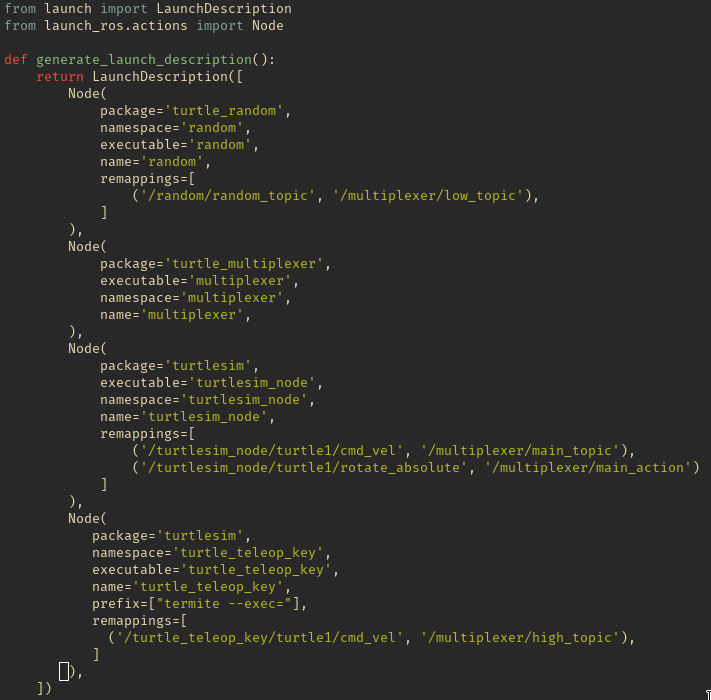
\includegraphics[width=0.3\linewidth]{images/ts_launch_file.png}
%\end{figure}
% Running the following ROS command \texttt{ros2 launch <file\_name>}, will automatically compile and run the launch file.

% By running the respective ROS \textit{launch} command, will automatically compile and run the launch file related to the \texttt{TurtleSim} example. Every network node is now running simultaneously in the background. The only foreground running node is the turtlesim one, because it has an associated interface showing the turtle movement.

% \begin{figure}[H]
%     \centering
%     \begin{minipage}{.6\textwidth}
%         \centering
%         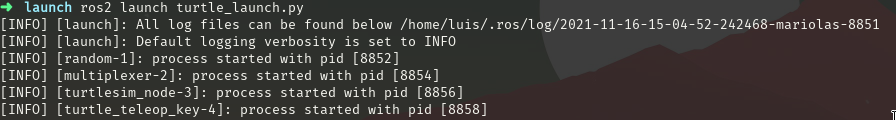
\includegraphics[width=\linewidth]{images/ts_launch_ros.png}
%         \caption{Nodes launched after running the launch file.}
%         \label{fig:ts-launch-sub}
%     \end{minipage}%
%     \begin{minipage}{.4\textwidth}
%         \centering
%         
\includegraphics[width=0.5\linewidth]{images/ts_turtle.png}
%         \caption{Turtlesim node interface.}
%         \label{fig:ts-turtle}
%     \end{minipage}
% 
%     \caption{Launching the \texttt{TurtleSim} network using a predefined launch file.}
%     \label{fig:ts-launch}
% \end{figure}

\begin{lstlisting}[title={\texttt{TurtleSim} launch file. Note that topic remap is used to properly address the transmission of movement commands from both publishers.}, language=xml]
<launch>
    <node name="turtlesim" pkg="turtlesim" exec="turtlesim_node" output="screen" args="-r /turtle1/cmd_vel:=/main_topic"/>
    <node name="keyboard" pkg="turtlesim" exec="turtle_teleop_key" args="--ros-args -r /turtle1/cmd_vel:=/high_topic"/>
    <node name="random" pkg="turtle_random" exec="random"/>
    <node name="multiplexer" pkg="turtle_multiplexer" exec="multiplexer"/>
</launch>
\end{lstlisting}

For understanding reasons, the reader may want to see how the network architecture is organized. ROS2 provides a GUI tool called \textit{rqt}, that assists developers in manipulating the network elements, in a more user-friendly manner. 

The \textit{rqt} visualizer, \textit{rqt\_graph}, allows the developer to perform analysis over a graphical visualization of the network computation graph.

\begin{figure}[H]
        \centering
        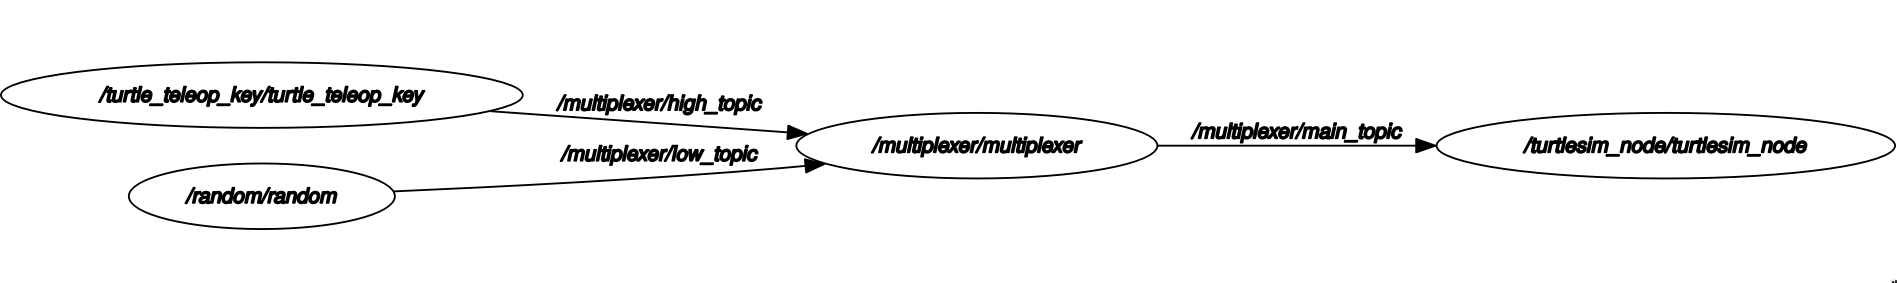
\includegraphics[width=0.8\linewidth]{images/ts_rqt_graph.png}
        \caption{\texttt{TurtleSim} network graph presented by \textit{rqt\_graph}.}
        \label{fig:ts-rqt-graph}
\end{figure}


The \textit{multiplexer} has two different active subscriptions, managing two different turtle movement values. Therefore, it must keep both subscriptions synchronized with each other. This is achieved by setting different priorities to each subscription. %, where the keyboard node has priority over the random controller, meaning that when the keyboard publishes movement data through its corresponding topic, the \texttt{multiplexer} must process that received data. 
\textit{Timers} are also used, since they provide a useful way of managing these topics, by time-assigning, alternately changing the priority after the timer runs out, through its corresponding callback function.

Based on the priority settled, the \textit{multiplexer} node forwards the commands through the \textit{main\_topic}, enabling the turtle movement. Every aspect related to the topic's publisher-subscriber pattern, in this ROS2 system, is treated over topic's namespace remapping.

\subsubsection{Services and Actions}

Even though \textit{topics} are the most conventional way of communication, due to its multicast scheme, subscribers can not be identified by the publishers, so logging and synchronization becomes rather difficult.

\textit{Services} allows a client, that can also be seen as a topic subscriber, to request data from a server, that likewise a topic publisher, furnish data through a service. The data is only provided when the client node makes a request. Each service is always linked to just one server node, and does not maintain active connections. To address the service stalling that the former ROS issued due to the service's synchronization nature, ROS2 services are asynchronous, since it is possible to specify a callback function that is triggered when the service server responds back to the client.

Other notable way of exchanging data is by setting goals through \textit{Actions}. Actions, likewise services, also uses a client-server model, but they were design for other purposes rather than only processing a request and sending back a response. Actions are intended to process long-running tasks, where the client sends a goal request to the server node, that confirms the receiving of this goal. Before returning a response back to the client, the server can send feedback back to the client. % Unlike services, actions can be cancelled, so the return response could not be acknowledge. A worth mentioned example, commonly used in robotic systems for navigation, is the intent of moving a robot to a position, previously requested by a client. While its traveling, it can send information about the transition state. When the robot reaches the predefined position, the server acknowledges the client by sending a result message.


\subsubsection{Parameters}   

Another relevant concept behind ROS is the existence of nodes \textit{parameters}, that allows individual configuration of the network nodes. In the former version of ROS, the node parameters were controlled by a global \textit{parameter server}, managed by its corresponding ROS Master. However, in ROS2 each node declares and manages its own parameters, by using the predefined commands \textit{get} and \textit{set}. Additionally, using a parameter function callback, the node's parameters can easily be edited.
        

\subsubsection{Node Composition}  

Usually a node is attached to a single process, but it is possible to combine multiple nodes into a single process, structurally abstracting some network parts, while improving the network's performance. However, there is a slight difference about how ROS and ROS2 approaches the node composition. In the former version of ROS, node composition was done over the combination of \textit{nodelets}, intentionally designed to ease the cost of overusing TCP for message-passing between nodes. Supported by the former idea of \textit{nodelets}, ROS2 introduces the \textit{components} as software code compiled into shared libraries, that can be loaded into a \textit{component container} process at runtime in the network, ensuring node composition. Node composition could also be applied for security matters. Suppose a scenario where multiple nodes respect the same security policies. By combining them into a single process, the mapping into this set of rules would be direct, easing the usage of security enclaves.
           

\section{Security}

The deployment of real-time systems implies critical concerning about safety and security \cite{maruyama2016exploring}, resulting of the demanding time-critical scenarios. Robotic systems fall under the umbrella of this broad system definition, as they feature unique cyber vulnerabilities related to its integration over highly networked environments, that confers great importance on exposing critical time-reliant scenarios. \cite{mcclean2013preliminary, dieber2017security} 

The network security evaluation in a system is done over applying several analyzing techniques. Generally, these techniques do not cover every security aspect, as new vulnerabilities arise from the technology evolution. \cite{kaeo2004designing}
The appliance of security countermeasures techniques upon configuring the system's network confers a critical step when aiming towards achieving security.

Within this vast topic, several different avenues of endeavor come to mind, each deserving of a substantial study. Network security entails pre-exploration of the system's network through practical networking security techniques, such as intrusion detection and traffic analysis. \cite{marin2005network} However, due to the high non-linearity and complexity of real-time systems, implementing such a thorough analysis method in near real-time remains a significant difficulty task. \cite{diao2009design}

% Future robotic systems will be situated in highly networked environments where they communicate with industrial control systems, cloud services or other sy- stems at remote locations. In this trend of strong digitization of industrial systems (also sometimes referred to as Industry 4.0), cyber attacks are an in- creasing threat to the integrity of the robotic systems at the core of this new development. It is expected, that the Robot Operating System (ROS) will play an important role in robotics outside of pure research-oriented scenarios. ROS however has significant security issues which need to be addressed before such products should reach mass markets. \cite{dieber2017security}

% System security concerning network exposure, often explored by unauthorized access and data leaking, can be treacherous and it is considered a complex subject, due to the abundance of different network security technologies that do not cover every security aspect, since absolute security does not exist, as new vulnerabilities arise from the technology evolution.\cite{kaeo2004designing} The appliance of security countermeasures techniques upon configuring the system's network confers a critical step when aiming towards achieving security. Within this vast topic, several different avenues of endeavor come to mind, each deserving of a substantial study. Network security entails pre-exploration of the system's network through practical networking security techniques, such as intrusion detection and traffic analysis. \cite{marin2005network}

% The concerns about security take on particular importance, since robots are becoming more frequently used and can directly affect the physical world. \textit{Cyber-physical} systems, commonly related to the arising of the automation concept of robots, feature unique vulnerabilities that exploit both cyber and physical nature of these devices. \cite{mcclean2013preliminary} Generally, when considering the deployment of a robotic system, the following information security pillars, over which attacking counter measures should be measured, are hopefully concerned: Confidentiality, Integrity and Availability. \cite{white2018procedurally}

\subsection{Security Integration in ROS2}

As aforementioned, ROS middleware faces known vulnerabilities due to its architecture model nature. The former ROS communication is built around TCP ports, allowing robots to be built as network distributed modules. As a result, techniques such as port scanning is usually used to expose the data itself. Due to the ROS master role in the communication architecture, and its ability to connect to other nodes, exposing this node poses a critical threat over the whole network. \cite{8794451} 

There was also worries regarding how ROS handled node communication. Network security may be jeopardized, as a result of the publish-subscribe pattern transparency, where node-to-node communications are settled in plain text, making data content vulnerable to unauthorized usage. \cite{kim2018security}

As result of the \textit{Data Distribution Service} (DDS) implementation as a flexible middleware interface in the ROS2 architecture, issues regarding security is no longer mainly ROS-dependent. Thus, when it comes to addressing security over communication, and subsequently data protection enhancment, ROS2 is heavily reliant on how the DDS standard is able to manage security. \cite{kim2018security, 8794451}

The \textit{Object Management Group} (OMG) \cite{3}, the already mentioned organization who is responsible for maintaining the DDS standard, accounts security integration by supplying an in-depth security specification, consequently adding features to the already developed DDS standard. The \textit{DDS-Security} is a specification that serves as a security extension to the DDS protocol, defined by a set of plugins (Authentication, Access Control, Cryptographic, Logging, Data Tagging), combined in a \textit{Service Plugin Interface (SPI)} architecture. \cite{8442103, ros-dds-integration}

\begin{figure}[H]
    \centering
    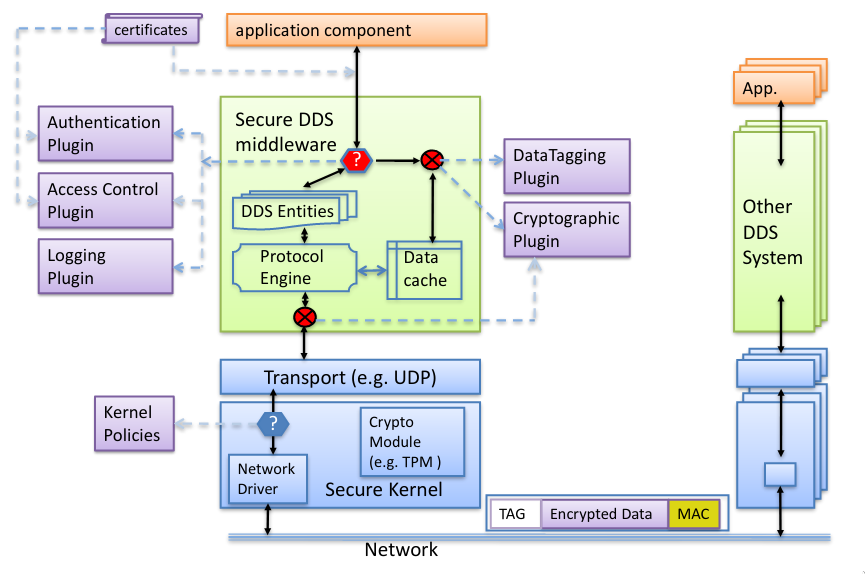
\includegraphics[width=0.7\linewidth]{images/dds-security-architecture.png}
    \caption{DDS-Security Architecture. Extracted from \cite{dds-s}.}
    \label{fig:dds-security-architecture}
\end{figure}

This specification enables its integration by furnishing a \textit{Security Model} supplied to the DDS standard, whereas the \textit{Service Plugin Interface} architecture is responsible for granting plugin enhancment for compliant DDS implementations. Moreover, depending on the security requirements needed for a particular application, these plugins might be adjusted by the latter's runtime DDS implementation. \cite{dds-s}

Every DDS implementation supported by ROS2 makes use of the DDS-Security specification, enabling security over ROS's application environment. Even though ROS2 is deployed without security mechanisms by default \cite{ros-dds-integration}, ROS2 provides a toolset, the \textit{Secure Robot Operating System 2} (SROS2) toolset, extending ROS2's functionality to make use of the DDS-Security functionality. 

The control over these tools are done by \textit{rcl}, providing security over the Application layer, while DDS is capable of providing security over the communication architecture. \cite{kim2018security} The SROS2 configuration is done over applying a set of security files to each ROS2 participant, considering the assignment approach (strict or permissive) that is being used.

Since this security integrity on ROS2 is consider a recent technology implementation \cite{ros-dds-integration}, the developer must be aware of improper configuration, that can still lead to security problems. However, the variety of capabilities in SROS2 toolset attempts to aid with security configuration across environments. 

\subsection{SROS2 Configuration}

To properly introduce the set of tools that SROS2 provides, the \texttt{TurtleSim} application already presented will now account the security features, as to provide authentication and encryption over the network communication, as well as access control policies over the application nodes. 
            
The \textit{multiplexer} node handles commands related to turtle's movement, acting as a topic selector between two different subscribed topics, each of them was respectively associated with a priority value. Based on the priority valued, the \textit{multiplexer} node forwards the commands, related to the selected topic, into the \textit{turtlesim} node, triggering the turtle's movement. 

However, \textit{multiplexer} is not exclusive to the \textit{turtlesim} node, as it is still possible to directly publish commands to the topic that handles the turtle's movement, since security policies are yet to be implemented.

% To accurately achieve this exclusivity, in which the turtle's movement is uniquely concerned by the \textit{multiplexer} node, \textit{access control} policies must be applied. The remaining nodes should be considered untrustworthy, denying any potential undesired turtle's movement. The idea is to encapsulate both \textit{multiplexer} and \textit{turtlesim} nodes, as the \textit{multiplexer} monitors and manages all data intended to manipulate turtle's movement.

%\begin{figure}[H]
%    \centering
%    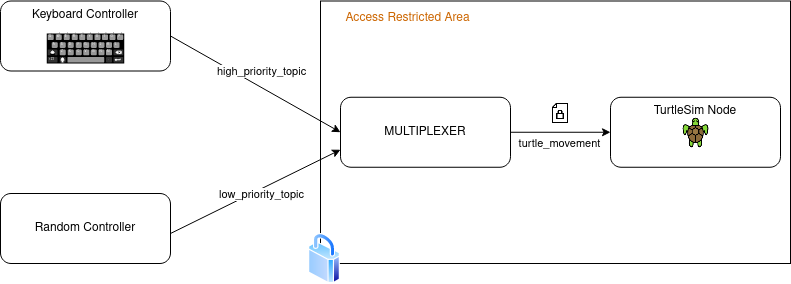
\includegraphics[width=0.8\linewidth]{images/ts_secured_multiplexer.png}
%    \caption{}
%    \label{fig:ts_secured}
%\end{figure}

% Note that, as it is now, the only nodes that are supervised by the \texttt{multiplexer} are the \texttt{random controller} node and the \texttt{keyboard} node. However, it can be implemented new nodes with ease, as it is only required to remap topics in the launch file and create as many subscriptions in the \texttt{multiplexer} as many implemented nodes.

In technically terms, a \textit{keystore} must be initiated beforehand, to provide a secured environment over the network. SROS2 yields a command that permits its creation. 

A keystore is a created directory where files regarding security are stored. By generating a keystore directory, it may then be sourced and utilized by \textit{rcl} features towards applying security to the application.
            
\begin{lstlisting}[title={\textit{Keystore} creation using the proper SROS2 command.}]
ros2 security create_keystore demo
\end{lstlisting}

The \textit{security} additional keyword-flag enables features regarding security matters, concerning the DDS-security artifacts.

\subsubsection{Keystore's Directory Architecture}

Upon the creation of the \textit{demo keystore}, three respective subdirectories are created, where each has their own role when it comes to security enhancment over the network.

\textbullet\  The \textit{enclaves} directory contains the security tools related to each enclave created. An \textit{enclave} is a group of ROS nodes, controlled by the same set of security rules, defined in its corresponding enclave directory. Each enclave includes files needed to enable security, such as CA certificates and their own private key (\texttt{key.pem}). % Besides containing each enclave created (for instance, in the figure above, a \texttt{/turtlesim/enclave} enclave is created), this directory also has a governance policy document \texttt{governance.xml}, as well as a signed copy file related to the CA permissions, \texttt{governance.p7s}. 

\textbullet\  The \textit{public} directory contains material that is permissible as public. A Certificate Authority certificate, \texttt{ca.cert.pem} is stored in this directory, related to the CA \textit{public key}. It is used to validate the identity and permissions of each ROS network node by the CA. DDS supports the separation of identity and permission chains, however ROS usually uses the former \texttt{ca.cert.perm} file, meaning that only a CA is used for both these processes.

\textbullet\  The \textit{private} directory contains material that is considered private. A Certificate Authority certificate, \texttt{ca.cert.pem} is stored in this directory, related to the CA \textit{private key}. It is used to modify the network policies, such as access permissions, and to add new participants. Similar to the public directory, the CA key corresponding to its identity and permissions can be stored in their corresponding individual directories.


The following exports need to be sourced to force SROS2 security features, as they concern relevant environment variables.

The first sourced variable points to the keystore's root, allowing ROS2 to identify where the security artifacts are kept. The second serves as the security enabler. The last variable sets which security strategy will be used when dealing with security files.
            
\begin{lstlisting}[title={SROS2 environment variables.}]
export ROS_SECURITY_KEYSTORE=/demo
export ROS_SECURITY_ENABLE=true
export ROS_SECURITY_STRATEGY=Enforce
\end{lstlisting}
            
\subsubsection{Understanding Security Enclaves}

Once the keystore has been created, the respective enclaves can be implemented. As mentioned, an enclave is a group of nodes that follow the same security policy. Enclaves usage are specified upon execution time, implying that their security artifacts are actually used by running processes.

Typically a node is an abstraction of a DDS \textit{participant}. However, by considering node composition, as a reliable way for matching multiple nodes simultaneously to the same enclave, this node perception as participants can not be taken into account, due to causing non-negligible overhead. There is also not convenient to compose nodes as individual participants, as far as operating system's security is concerned, where permission distribution and memory becomes rather difficult to handle.

To adress this, each participant must be matched to a node shared context, instead of being directly related to a specific node. Thereby, the initial given definition of an enclave is not totally correct, since a participant can either be perceived as single node or as multiple node shared context. So, each enclave security artifacts are used by its respective DDS participant. 

As long as security is enabled, the whole networt must be properly authenticated. Thus, every node within the network must be authenticated, using an enclave as their identifier. Node composition can not be considered in this network, as it is not intended to share topic privileges. Note that, if an enclave was shared by multiple nodes, each node policy would be consider as common policy within the enclave.

\begin{lstlisting}[title={\texttt{TurtleSim} enclave creation.}]
ros2 security create_key demo /turtlesim
ros2 security create_key demo /multiplexer
ros2 security create_key demo /keyboard
ros2 security create_key demo /random
\end{lstlisting}

The keystore creation, alongside with their respective enclaves, only ensures security over the network communication, in which node authentication and data encryption are concerned. With the proper use of port scanning tools, data encryption can be easily verified. Authentication is ensured upon the enclave's creation. However, to properly apply security over the \texttt{TurtleSim} application, acess control policies must be appropriately covered.

\subsubsection{Access Control}

To accurately achieve topic exclusivity, in which the turtle's movement is uniquely concerned by the \textit{multiplexer} node, \textit{access control} policies must be applied. The remaining nodes should be considered untrustworthy, denying any potential undesired turtle's movement.
            
In order to provide access control, each permission file needs to be modified, accounting the network policies restrictions. This is ensured by adding security permissions to these files, with the mandatory signature of the Certificate Authority. A suitable way of editing the permission file, \textit{permissions.xml} (file that dictates how the enclave manages the permissions within the network) is by creating a policy file, that restrictly specify the set of permissions of each enclave.

Following the \textit{ConArmor} policy language \cite{white2018procedurally}, the \textit{SROS2 policy file} confers a restrict \textit{XML schema}, where security policies bind profiles to access permissions for network objects, granting privileges back to a certain profile. \textit{Profiles} are implemented under the \textit{enclave} declaration, to duly support the node composition into a single process, enabling the possibility of combining multiple profiles, respectively addressing its corresponding node. Typically, each \textit{enclave} declaration is linked to a corresponding ROS node, naturally perceived as a DDS participant. 

\textit{Objects} are classified over a subsystem type, structurally characterized by permissions tags. Then \textit{object privileges} are controlled over access values, either \textit{allow} or \textit{deny}, attributed to their corresponding permissions tags. For instance, consider the \textit{topics} domain, where a profile can either publish or subscribe to that topic. To properly address the allowance of a profile privilege over a topic, the permission tag (either subscribe or publish) must be followed with the \textit{allow} tag.

The policy design approach works under the \textit{Mandatory Access Control} (MAC), that denys any privilege by default. The only way of allowing access to any object, is by explicitly specifying the subject's privilege access. 

\begin{lstlisting}[title={Setting permissions into each enclave.}]
ros2 security create_permission demo /turtlesim policies.xml
ros2 security create_permission demo /multiplexer policies.xml
ros2 security create_permission demo /keyboard policies.xml
ros2 security create_permission demo /random policies.xml
\end{lstlisting}

As it follows, security is enabled within this network as well as policy control over topic's permissions. The network can be easily configured and automatically launched through the execution of a launch file, where \textit{roslaunch} uses this files to perform overall initialization.

\begin{lstlisting}[title={\texttt{TurtleSim} launch file. Note that topic remap is used to properly address the transmission of movement commands from both publishers.}, language=xml]
<launch>
    <node name="turtlesim" pkg="turtlesim" exec="turtlesim_node" output="screen" args="--ros-args --enclave /turtlesim -r /turtle1/cmd_vel:=/main_topic" />
    <node name="keyboard" pkg="turtlesim" exec="turtle_teleop_key" output="screen" args="--ros-args --enclave /keyboard -r /turtle1/cmd_vel:=/high_topic" />
    <node name="random" pkg="turtle_random" exec="random" args="--ros-args --enclave /random" />
    <node name="multiplexer" pkg="turtle_multiplexer" exec="multiplexer" args="--ros-args --enclave /multiplexer" />
</launch>
\end{lstlisting}

The network is now sucessfully running as a secured environment, where nodes within this network can not be perceived from outside, neither their topic list. To prove that access control is properly employed, the user may want to try to enhance the turtle movement directly from the random controller, by forcing the remapping of the \textit{low\_topic} to the \textit{main\_topic}.  Thus, by attempting to remap the \textit{low\_topic} topic prevents the node from launching, since random is only allowed to publish through the \textit{low\_topic}. 

\begin{lstlisting}[title={Attempting the \textit{low\_topic} remap.}, language=xml]
<node name="random" pkg="turtle_random" exec="random" args="--ros-args --enclave /random -r /low_topic:=/main_topic"/>
\end{lstlisting}

However, if the user forces the inverted remap, it is possible to control the turtle movement directly from the random controller, since no policie has been disrespecteded. Although, the random controller is still publishing to the \textit{low\_topic}, the \textit{main\_topic} in which the turtle movement is concerned is remapped towards the \textit{low\_topic}. This concerns a problem that is not been duly address by the ROS community. It is unreasonable to expect this flexibility in a secured network, since policies initially settled can be easily compromised.